%!TEX root = ../Main.tex

% -----------------------------------------------------------------------------
\section{Implementation}
\label{s:Evaluation}

Stream fusion is ultimately performed for practical reasons: we want the fused result program to run faster than the original unfused program.


% -----------------------------------------------------------------------------
\subsection{Finite streams}
\label{s:Finite}

The processes we have seen so far deal with infinite streams, but in practice most streams are finite. Certain combinators such as @fold@ and @append@ only make sense on finite streams, and others like @take@ produce inherently finite output. We have focussed on the infinite stream version as it is simpler to explain and prove, but supporting finite streams does not require substantial conceptual changes.

Unlike infinite streams, pulling from a finite stream can fail, meaning the stream is finished. We therefore modify the @pull@ instruction to have two output labels: one to execute when a value is pulled, and the other to execute when the stream is finished. On the pushing end, we also need some way of finishing streams, so we add a new instruction to close an output stream.

During evaluation we need some way of knowing whether a stream is closed, which can be added as an extra constructor in the \InputState~ type. The same constructor is added to the static input state used by fusion. In this way, for any changes made to evaluation, the analogous static change must be made in the fusion transform.

It is also possible to encode finite streams as infinite streams with an explicit end-of-stream marker (EOF) and case statements. However, this requires the fusion transform to reason about case statements' predicates.
By making the structure of finite streams explicit and constraining how processes use finite streams, it is not necessary to rely on heuristics for deciding equality of predicates.

% Waffle waffle to get url on its own line
This finite stream extension is described in more detail in the appendix of the extended version of this paper, which is available at \url{http://cse.unsw.edu.au/~amosr/papers/merges.pdf}.

% It seems obvious that if two consumers read the same value and check if it is EOF, they will both be the same, but this is undecidable in general.


% -----------------------------------------------------------------------------
\subsection{Benchmarks}
We have implemented this system using Template Haskell in a library called @folderol@\footnote{\url{https://github.com/amosr/folderol}}.
To show practical examples, we use the finite stream extension mentioned in~\S\ref{s:Finite}.
We present three benchmarks: two file-based benchmarks, and one array algorithm.

For the file benchmarks, we compare against three Haskell streaming libraries: `Conduit', `Pipes', and `Streaming'.
These streaming libraries are pull-based, and do not naturally support multiple outputs: the split in the dataflow graph must be hand-fused, or somehow rewritten as a straight-line computation.
These libraries also have a monadic interface, which allows the structure of the dataflow graph to depend on the values. This expressiveness has a price: if the dataflow graph can change dynamically, we cannot statically fuse it.
% This price is paid even when the dataflow graph is static, as the same monadic structure is used: because repetition is expressed as an unfolding dynamic graph, even computations that would be static in other systems must be expressed dynamically, reducing the possibility for fusion.

The first file benchmark simply appends two files while counting the lines.
In Pipes and Conduit, counting the lines is implemented as a pipe which counts each line before passing it along.
The first group in Figure~\ref{fig:bench:all} shows the runtimes for appending 2MB of data.

The second file benchmark takes a file and partitions it into two files: one with even-length lines, and one with odd-length lines.
The output lines are also counted.
Even with partial hand-fusion because of the multiple outputs, the Pipes and Conduit programs are slower than ours, as well as losing the abstraction benefits from using a high-level library.
The `Streaming' library allows streams to be shared in a fairly straightforward way and does not require hand-fusion, but is also the slowest in this benchmark.
The second group in Figure~\ref{fig:bench:all} shows the runtimes for partitioning a 1MB file.


Quickhull is a divide-and-conquer spatial algorithm to find the smallest convex hull containing all points.
At its core is an operation called `filterMax' which takes a line and an array of points, and finds the farthest point above the line, as well as all points above the line.

Here we also compare against a @Data.Vector@ program, which uses shortcut fusion.
The shortcut fusion system cannot fuse both operations into a single loop, and both operations must recompute the distances between the line and each point.
% This means a choice must be made: either compute the distances upfront and share them, or recompute the distances in each operation.
% We compared both, and recomputing was significantly faster.
% However, we only benchmarked with two-dimensional points: at higher dimensions, the cost of recomputing distances may outweigh array allocation.
As before, the Conduit and Pipes programs must be partially hand-fused.
The third group in Figure~\ref{fig:bench:all} shows the runtimes for Quickhull over 40MB of data, or half a million points, while the final group uses more data (120MB) to compare directly against @Data.Vector@.


% -----------------------------------------------------------------------------
\subsection{Optimisation and Drop Instructions}
\label{s:Optimisation}
After we have fused two processes together, it may be possible to simplify the result before fusing in a third. Consider the result of fusing @group@ and @merge@ which we saw back in Figure~\ref{fig:Process:Fused}. At labels @F1@ and @F2@ are two consecutive @jump@ instructions. The update expressions attached to these instructions are also non-interfering, which means we can safely combine these instructions into a single @jump@. In general, we prefer to have @jump@ instructions from separate processes scheduled into consecutive groups, rather than spread out through the result code. The (PreferJump) clauses of Figure~\ref{fig:Fusion:Def:StepPair} implement a heuristic that causes jump instructions to be scheduled before all others, so they tend to end up in these groups.

Other @jump@ instructions like the one at @F5@ have no associated update expressions, and thus can be eliminated completely. Another simple optimization is to perform constant propagation, which in this case would allow us to eliminate the first @case@ instruction. 

Minimising the number of states in an intermediate process has the follow-on effect that the final fused result also has fewer states. Provided we do not change the order of instructions that require synchronization with other processes (@pull@, @push@ or @drop@), the fusibility of the overall process network will not be affected.

% Another optimization is to notice that in some cases, when a heap variable is updated it is always assigned the value of another variable. In Figure~\ref{fig:Process:Fused}, the @v@ and @x1@ variables are only ever assigned the value of @b1@, and @b1@ itself is only ever loaded via a @pull@ instruction. Remember from \S\ref{s:Fusion:FusingPulls} that the variable @b1@ is the stream buffer variable. Values pulled from stream @sIn1@ are first stored in @b1@ before being copied to @v@ and @x1@. When the two processes to be fused share a common input stream, use of stream buffer variable allows one process to continue using the value that was last pulled from the stream, while the other moves onto the next one. 

When the two processes are able to accept the next variable from the stream at the same time, there is no need for the separate stream buffer variable. This is the case in Figure~\ref{fig:Process:Fused}, and we can perform a copy-propagation optimisation, replacing all occurrences of @v@ and @x1@ with the single variable @b1@. To increase the chance that we can perform copy-propagation, we need both processess to want to pull from the same stream at the same time. Moving the @drop@ instruction for a particular stream as late as possible prevents a @pull@ instruction from a second process being scheduled in too early.

% In the result, the interleaved instructions from both source processes then share the same heap variable.  

% In general, the @drop@ for a particlar stream should be placed just before a @pull@ from the same stream. 
\begin{figure}
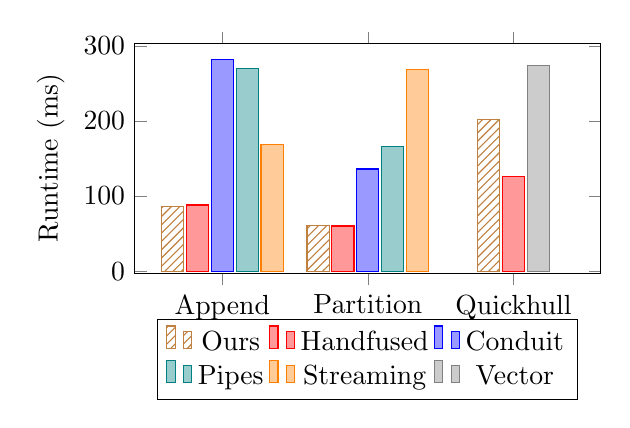
\begin{tikzpicture}
\usetikzlibrary{patterns}

% Bar chart for benchmarks:
% This is a complicated bar chart because there are six series (conduit, pipes, vector..), but they are not all defined at all points (append, partition, quickhull).
% We need to split it into three different pictures, overlaid on top of each other.
% The first picture just defines the legend, the axis labels, etc.
\begin{axis}[
  symbolic x coords={Append, Partition, Quickhull, end},
  xtick=data, ylabel=Runtime (ms),
  % All pictures need to specify same upper and lower bounds so they line up together
  ymin=0, ymax=300,
  xmin=Append, xmax=Quickhull,
        enlargelimits=0.01,
  enlarge x limits=0.30,
        ybar=1pt,
        bar width=8pt,
  width=7.5cm, height=4.5cm,
  legend style={at={(0.5,-0.2)},anchor=north, legend columns=3},
]
% The colours need to be specified manually, to force the legend entries to show up..
% The colours also need to match the colours specified for each series data.
\addlegendimage{brown,pattern=north east lines,pattern color=brown}
\addlegendimage{red,fill=red!40!white}
\addlegendimage{blue,fill=blue!40!white}
\addlegendimage{teal,fill=teal!40!white}
\addlegendimage{orange,fill=orange!40!white}
\addlegendimage{gray,fill=gray!40!white}
\legend{Ours, Handfused, Conduit, Pipes, Streaming, Vector}
\end{axis}

% This picture shows the values for Append and Partition, since they have the same series defined
\begin{axis}[
  symbolic x coords={Append, Partition, Quickhull, end},
  ticks=none,
  ymin=0, ymax=300,
  xmin=Append, xmax=Quickhull,
  enlargelimits=0.01,
  enlarge x limits=0.30,
  ybar=1pt,
  bar width=8pt,
  width=7.5cm, height=4.5cm,
]
% Ours
\addplot[brown,pattern=north east lines,pattern color=brown] coordinates {(Append,  86) (Partition,  61)   };
% Handfused
\addplot[red,fill=red!40!white] coordinates {(Append,  88) (Partition,  60)   };
% Conduit
\addplot[blue,fill=blue!40!white] coordinates {(Append, 282) (Partition, 136)   };
% Pipes
\addplot[teal,fill=teal!40!white] coordinates {(Append, 270) (Partition, 166)  };
% Streaming
\addplot[orange,fill=orange!40!white] coordinates {(Append, 168) (Partition, 268)  };
\end{axis}

% This picture shows the Quickhull results
\begin{axis}[
  symbolic x coords={Append, Partition, Quickhull, end},
  ticks=none,
  ymin=0, ymax=300,
  xmin=Append, xmax=Quickhull,
  enlargelimits=0.01,
  enlarge x limits=0.30,
  ybar=1pt,
  bar width=8pt,
  width=7.5cm, height=4.5cm,
]
% Ours
\addplot[brown,pattern=north east lines,pattern color=brown] coordinates {  (Quickhull, 202)  };
% Handfused
\addplot[red,fill=red!40!white] coordinates {  (Quickhull, 126)  };
% Vector
\addplot[gray,fill=gray!40!white] coordinates {(Quickhull, 274)  };
\end{axis}

% Runtimes for Quickhull 40MB:
% Conduit 2-pass:     300ms
% Conduit 1-pass:     264ms
% Hand:                 3ms
% Folderol:             6ms
% Vector recompute:     8ms
% Vector store:        11ms

\end{tikzpicture}
\caption{Runtime for benchmarks; lower is faster.}
\label{fig:bench:all}
\end{figure}



